\documentclass[12pt]{article}

\usepackage{url}
\usepackage{hyperref}
\usepackage[margin=1in]{geometry}
\usepackage{cite, enumerate, amsmath, amssymb}
\usepackage{graphicx}

\graphicspath{ {images/} }

%%%%%%%%%%%%%%%%%%%%%%%%%     CODE LATEX     %%%%%%%%%%%%%%%%%%%%%%%%%%%%
\usepackage{color}
\usepackage{xcolor}
\definecolor{bluekeywords}{rgb}{0.13,0.13,1}
\definecolor{greencomments}{rgb}{0,0.5,0}
\definecolor{redstrings}{rgb}{0.9,0,0}
\definecolor{light-gray}{gray}{0.95}

\usepackage{listings}
\newcommand{\MYhref}[3][blue]{\href{#2}{\color{#1}{#3}}}%

\definecolor{dkgreen}{rgb}{0,0.6,0}
\definecolor{gray}{rgb}{0.5,0.5,0.5}
\definecolor{mauve}{rgb}{0.58,0,0.82}

\lstdefinelanguage{Shell}{
  keywords={tar, cd, make},
  keywordstyle=\color{dkgreen}\bfseries,
  alsoletter={+},
  ndkeywords={python, py, javac, java, gcc, c, g++, cpp, .txt, .tar},
  ndkeywordstyle=\color{dkgreen}\bfseries,
  identifierstyle=\color{black},
  sensitive=false,
  comment=[l]{//},
  morecomment=[s]{/*}{*/},
  commentstyle=\color{purple}\ttfamily,
  stringstyle=\color{red}\ttfamily,
  morestring=[b]',
  morestring=[b]"
}

\lstset{
  basicstyle=\ttfamily,
  columns=fullflexible,
}
\lstset{columns=fullflexible, basicstyle=\ttfamily,
    backgroundcolor=\color{light-gray},xleftmargin=0.5cm,frame=tlbr,framesep=4pt,framerule=0pt}
%%%%%%%%%%%%%%%%%%%%%%%%%%%%%%%%%%%%%%%%%%%%%%%%%%%%%%%%%%%%%%%%%%%%%%%%%%

\providecommand{\abs}[1]{\left\vert#1\right\vert}
\providecommand{\norm}[1]{\left\Vert#1\right\Vert}

\begin{document}

\title{
    \normalsize Final Project Report for 15-418, Spring 2018: \\
    \LARGE A Parallel Sketching Library for GPUs
}
\author{Eliot Robson \qquad Taisuke Yasuda\\ \small
\href{mailto:erobson@andrew.cmu.edu}{erobson@andrew.cmu.edu} \quad \href{mailto:taisukey@andrew.cmu.edu}{taisukey@andrew.cmu.edu}}

\maketitle

\begin{abstract}
	In this course project, we implemented and optimized matrix sketching algorithms on CPU in C++ and in CUDA on the GPU, as well as stream sketching algorithms in C++ with OMP. We mainly measured for leverage score sampling sketch for the CUDA sketches, for which we achieve as high as $40\times$ speedup, and modified absorption sketch for the OMP sketches, for which we achieve as high as $8\times$ speedup.
\end{abstract}

\section{Background}
Sketching algorithms are a class of randomized approximation algorithms designed to approximate large matrices with ones with less rows and/or columns. These algorithms are known to have provable approximation guarantees with high probability and can be applied to countless downstream applications for asymptotically faster approximation algorithms, including but most certainly not limited to linear regression, low rank approximations, and preconditioning. We refer the audience to a monograph by David Woodruff for an excellent overview of sketching algorithms \cite{woodruff2014sketching}, especially as applied to linear algebraic operations.

We describe more specifically what sketching looks like. In theory, all our sketches are linear and take the form of a random matrix $S$ sampled from some distribution over $\mathbb R^{p\times n}$. When we use this to sketch a large matrix $A\in\mathbb R^{n\times d}$, we create
\[
	SA\in\mathbb R^{p\times d},
\]
where $p\ll n$ and thus $SA$ has much fewer rows than $A$. As mentioned above, the point of sketching algorithms is to approximate matrices with smaller ones. Of course, we need to be precise in describing what the ``approximation'' guarantees. In the theoretical literature, a standard approximation guarantee is a subspace embedding, so this is what we guarantee in our library, with probability of success at least $99/100$. The subspace embedding guarantee is that we preserve distances up to a $(1\pm\varepsilon)$ multiplicative factor, where $\varepsilon>0$ is a given measure of accuracy. Written in math, this is the guarantee that with probability at least $99/100$, we have that
\[
	\norm{SAx}_2^2 = (1\pm\varepsilon)\norm{Ax}_2^2
\]
for all $x\in\mathbb R^d$, where the norm above is the standard Euclidean norm. Note that there are a whole variety of other types of approximation guarantees, such as matrix product guarantees, projection cost preservation, etc. However, we stick to just the subspace embedding guarantee for now. Thus, we expose the following interface for our library:
\begin{lstlisting}
class sketch_interface {
	public:
		sketch_interface(size_t p, size_t n);
		void sketch(matrix *A, matrix *SA);
		size_t eps_approx_rows(size_t n, size_t d, double eps);
}
\end{lstlisting}
where \texttt{eps\_approx\_rows} returns the number of rows $p$ needed for the sketch $S$ to give a subspace embedding with probability at least $99/100$. 

The sketching library that we have implemented currently supports three general matrix sketching algorithms: Gaussian sketch, count sketch, and leverage score sampling sketch. These sketching algorithms are implemented as the classes \texttt{gaussian\_sketch}, \texttt{count\_sketch}, and \texttt{leverage\_score\_sketch} and inherit from the above interface. The Gaussian sketch and count sketch are extremely straightforward algorithms that are extremely easily parallelized. They are extremely useful as standalone sketching algorithms, but the main reason for their implementation is that they are used as a subroutine for the much more advanced leverage score sampling. We now describe the algorithms implemented in our library in more detail. 

\subsection{Gaussian Sketch}
The Gaussian sketch is extremely simple, for a specified number of rows $p$ for the sketch, we sample a $p\times n$ matrix of IID Gaussians with mean $0$ and variance $1/p$. This is the construction for the famous Johnson-Lindenstrauss lemma in the form of a randomized algorithm, rather than a probabilistic existence statement. Since the sketch is just a multiplication by a dense matrix, there is not much we can do to speed this algorithm up besides general tricks for matrix multiplication. For a $(1+\varepsilon)$ subspace embedding, we just need
\[
	p\geq 4\left(\frac{\varepsilon^2}2-\frac{\varepsilon^3}3\right)^{-1}\log n
\]
rows, a proof for which can be found in \cite{dasgupta2003elementary}, for example.

\subsection{Count Sketch}
Count sketch is a slightly more sophisticated sketching algorithm that is extremely sparse: it only has one nonzero entry for every column. Thus, it can be stored and applied very quickly. In return, we pay for a larger value of $p$ for a subspace embedding. The sketching matrix $S$ is formed as follows: for each of the $n$ columns of the $p\times n$ matrix $S$, uniformly randomly select one of the $p$ indices, and uniformly choose an entry from $\{1,-1\}$. For instance, a $4\times 5$ count sketch matrix might look like:
\[
	\begin{pmatrix}
		0 & 0 & -1 & 1 & 0 \\
		1 & 0 & 0 & 0 & 0 \\
		0 & 0 & 0 & 0 & 1 \\
		0 & -1 & 0 & 0 & 0
	\end{pmatrix}
\]
For the number of rows $p$, we refer to lecture slides by David Woodruff, found at \url{http://www.cs.cmu.edu/afs/cs/user/dwoodruf/www/teaching/15859-fall17/weekTwo.pdf}, which provides a proof for
\[
	p\geq \frac{6d^2}{\delta\varepsilon^2}
\]
where $\delta$ is a bound on the error probability. 

We now the describe the dependency structure for this algorithm. Essentially, the algorithm looks at each row of the input matrix $A$, chooses a random sign to scale it by, and copies the result to a random row index $j\in[p]$. Since the rows of the matrix $A$ are moved together to the same location of the sketched matrix $SA$, the columns are dependent within a single row. However, the rows are independent and thus the sketched result can be computed independently for blocks of rows and then combined later by linearity of the sketch. 

\subsection{Leverage Score Sampling}
We finally discuss a sketching algorithm based on sampling. Uniformly sampling the rows of a matrix is a very intuitive way of forming an approximation to the matrix, but unfortunately, fails to give theoretical guarantees. The problem is that in order to capture the essence of a matrix, one needs to make sure to capture a small number of rows that are ``outliers'' in some sense, but uniform sampling will not capture these rows with high enough probability. However, sketches based on sampling are desirable for many reasons. For instance, the sketches discussed will yield dense matrices in general, even if the input matrix is sparse. However, sampling-based sketches will preserve sparsity. In addition, sampling-based sketches are more interpretable, as the rows are rows from the original matrix themselves, not some linear combination. 

The way to make sampling work as a sketch is to sample proportionally to the \emph{leverage scores} of a matrix, which are the norms of the left singular vectors of the matrix (columns of $U$ where $A = U\Sigma V^\top$ is the singular value decomposition). Note that exact computation of the leverage scores is not compatible with a sketching algorithm, since this takes way too long and defeats the purpose of computing the sketch. Thus, we employ a fast approximation algorithm to obtain constant factor estimates of the leverage scores, which can then be used to obtain the leverage score sampling sketch. The approximation of the leverage scores is based on other subspace embedding sketches -- this is where we use our Gaussian sketch and count sketch from before. The pseudocode for the algorithm for fast approximation of leverage scores is given as follows:
\begin{enumerate}
	\item Compute a count sketch $SA$ of the input matrix $A$
	\item Compute a factorization $SA = QR^{-1}$ so that $Q$ is orthonormal
	\item Compute $R$, the inverse of $R^{-1}$
	\item Compute a Gaussian sketch $RG$ of $R$
	\item Compute $A(RG)$
	\item Compute the row norms times a scalar factor
\end{enumerate}
Then, we obtain a $(1+\varepsilon)$ subspace embedding sketch based on sketching by sampling $p$ times, where
\[
	p\geq \frac{C\cdot \frac43\frac{d}{\beta}\log d}{\varepsilon^2}
\]
for which $\beta = 4/7$ and 
\[
	2de^{-C6d\log d/6d} = 2de^{-C\log d} = 2d^{1-C}<\frac1{100}\impliedby d^{C-1}>200\iff C = 1 + \log_d 200.
\]
These numbers were obtained by tracking constants for the proof given in lecture slides by David Woodruff (\url{http://www.cs.cmu.edu/afs/cs/user/dwoodruf/www/teaching/15859-fall17/weekFour.pdf}). 

This algorithm is the main algorithm that benefits greatly from running on a GPU, since it is quite computationally intensive in exchange for sparsity and interpretability of the resulting sketch. As described in more detail in the section \ref{approach-leverage}, we can reveal independence structure from the algorithm after taking the QR decomposition, which allows us to decouple the columns of $R$ when we compute the inverse of $R^{-1}$, along with subsequent computations. 

\section{Approach}
Our baseline sequential implementation for our matrix sketching algorithms was developed in C++, using the linear algebra library Eigen (\url{https://eigen.tuxfamily.org/}). Our optimized GPU implementation was developed in CUDA on NVIDIA GPUs, making use of the CUDA helper libraries CUBLAS, CUSOLVER, and CURAND. As great as CUBLAS is, CUBLAS routines cannot be called on shared memory, and thus we still have a lot of optimization left on the table that could be collected by rewriting some of the CUBLAS routines manually to operate on shared memory. Instead, when we call CUBLAS routines from device functions, child kernels are spawned from these parent kernels, and we content ourselves with optimization due to just parallelism and locality without the speed of shared memory. 

\subsection{Leverage Score Sampling}\label{approach-leverage}
At first glance, the algorithm seems to suffer from a lot of dependencies, as the algorithm involves a lot of matrix operations both from the left and right. Another level of complexity is added by the fact that CUBLAS, the CUDA basic linear algebra subroutines library, is written to execute everything in column major order. We carefully describe from an implementation point of view how to milk out all the independent components to this algorithm.

\subsubsection{Sampling Gaussians}
First note that we can start the expensive sampling of the Gaussian matrix $G$ at the very beginning in parallel and hide the latency using the time it takes to do the expensive linear algebraic computations that forms the core of the algorithm. In addition, although we may simply sample the matrix as a $d\cdot O(\log n)$ matrix, we may access the columns in any order that is friendly to the cache as long it is consistent with using a permutation of the Gaussian matrix, since the entries are just IID random variables. We will come back to this later, so keep this in mind. 

\subsubsection{QR Decomposition}
We describe our strategy for computing $R^{-1}$ efficiently. The most important observation is that we can factor the matrix $SA$ using a QR factorization algorithm, which gives us an orthonormal matrix $Q$ as desired as well as the matrix $R^{-1}$ that is \emph{upper triangular}. Although this was likely an obvious observation for researchers in the numeric linear algebra community, it took us a while to make use of this fact since we learned about this algorithm in a theory class, which only emphasized the fact that $Q$ was orthonormal (the more important fact when proving correctness). We make use of the CUSOLVER routine \texttt{geqrf} to compute this QR factorization. Note that when computing $R$, we just want to solve for the matrix $X$ such that
\[
	R^{-1}X = I.
\]
This is efficient when $R^{-1}$ is upper triangular, since the computation is now just back substitution to solve for a single column. Since CUBLAS has an efficient implementation of solving triangular systems of equations, \texttt{trsm}, we use this. 

\subsubsection{Load-Balancing the Computation of $R$}
However, our profits from doing the QR factorization go beyond just this. Observe that when solving the upper triangular system $R^{-1}x = e_i$ in order to find the $i$th column of $R$, we immediately find that $x_j = 0$ for all $i < j\leq n$ (this is used to show that the inverse of an upper triangular matrix is also upper triangular). Thus, the computation of the $i$th column of $R$ only depends on the first $i$ columns of $R^{-1}$. Fortunately, CUBLAS operates in column major order, so we can efficiently copy out the first $i$ columns, as these are contiguous in memory. This also helps us do some load balancing: we know that the last columns of $R$ take longest to compute, while the first columns are instantaneous. Thus, the best way to assign the work is as follows: if we have $T$ threads computing $R$, then we should divide the columns of $R$ into $2T$ blocks $B_1, B_2,\dots, B_{2T}$, and assign blocks $B_t$ and $B_{2T-t+1}$ to thread $t\in[T]$.

\subsubsection{Split Counters and $G$ Layout Tricks for Computation of $RG$}
At this time, recall that the columns of $R$ corresponding to column blocks $B_t$ and $B_{2T-t+1}$ reside on thread $t$. The next step is to compute $RG$. This is the step in which we play with the interpretation of the matrix $G$. Note that each of the $O(\log n)$ columns of $G$ specifies a linear combination of the columns of $R$. Then, we can precompute the partial sum of this linear combination, just for the columns of $B_t$ and $B_{2T-t+1}$ that reside on thread $t$, and put them together at the end by linearity, similar to how split counters can be used to accumulate partial counts. Then, to do this, we only see the rows of $G$ corresponding to $B_t$ and $B_{2T-t+1}$, and furthermore, we can take them to be contiguous in memory, and even only resident on thread $t$ since these rows are only used by thread $t$. Thus, we can minimize communication between threads this way.

\subsubsection{Computation of Approximated Leverage Scores}
In the final step for computing the approximated leverage scores, we must combine $RG$ into one matrix since the row norms of $ARG$ must be computed. However, once $RG$ is computed, $A$ can be split up into row blocks and the $i$th leverage score estimate
\[
	\ell_i := \frac{\beta}{d}\norm{(e_i^\top A)(RG)}_2^2
\]
can be computed independently. In addition, we will need the CDF for sampling later, for which we can precompute the partial sums as in split counters. 

\subsubsection{Sampling and Applying the Sketch}
The last step is to sample according to the distribution and apply the sketch, but these are easily parallelized.

\section{Results}

\subsection{Leverage Score Sampling}
We first present our results for implementing leverage score sampling on GPUs. Correctness of our algorithms were ensured by checking that our graphs were indeed a subspace embedding, i.e.\ that for random vectors, the Euclidean norms were preserved. 

Our benchmark data was derived from a range of randomly generated matrices, ranging from around a few kilobytes ($10\times 5$ matrices) up to around 40 megabytes ($30000\times 100$ matrices). To measure the efficiency of our CUDA implementation, we compared the time to a single-threaded C++ implementation based on optimized linear algebra subroutines of the Eigen library. We computed the wall-clock time of both the sequential and parallel implementations and took the ratio of the sequential time and the parallel time to be our speedup. 

\begin{figure}[ht]
\centering
\label{speedup-vs-rows}
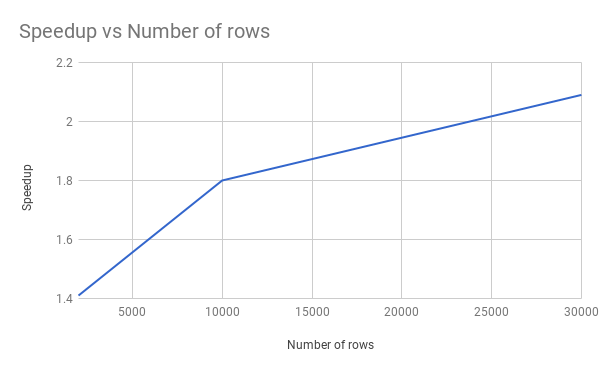
\includegraphics[scale=0.7]{speedup-vs-rows}
\caption{Speedup does not improve as a function of $n$}
\end{figure}

\begin{figure}[ht]
\centering
\label{speedup-vs-cols}
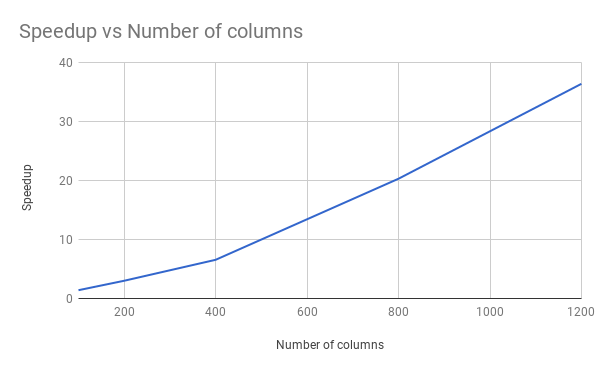
\includegraphics[scale=0.7]{speedup-vs-cols}
\caption{Speedup improves dramatically as a function of $d$}
\end{figure}

\begin{figure}[ht]
\centering
\label{speedup-vs-threads}
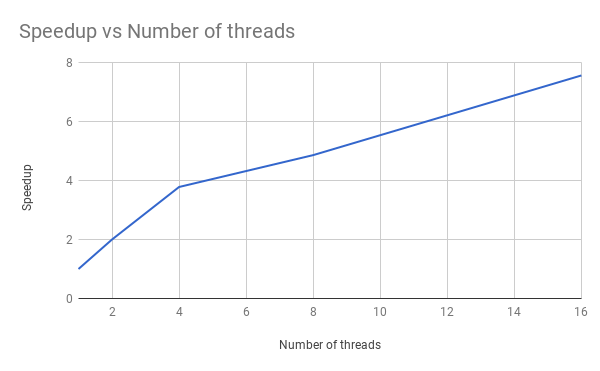
\includegraphics[scale=0.7]{speedup-vs-threads}
\caption{Speedup improves dramatically as a function of $d$}
\end{figure}

\section{Division of Work}
Equal work was performed by both project members. 

\nocite{talukdar2014scaling}
\nocite{talukdar2009new}

\bibliographystyle{alpha}
\bibliography{citations}

\end{document}